% =========================================================================
% Secao 4 - Resultados agregados Brasil
% =========================================================================

\section{Resultados agregados para o Brasil}
\label{sec:agregados}

A Tabela~\ref{tab:t1_brasil} reporta os indicadores de fluxo escolar
para o Brasil, por macroetapa e ano calendário, no período
2012--2023. As taxas inter-ano são calculadas com a metodologia
descrita na Seção~\ref{ssec:definicoes}, em que a observação de
referência em $t$ e em $t+1$ é tomada entre os trimestres $Q_2$ e
$Q_3$ de cada ano, usando o máximo do nível educacional declarado.
A taxa de abandono é calculada na subamostra dos alunos com
observação nos quatro trimestres do mesmo ano e é reportada
separadamente na Tabela~\ref{tab:abandono_fullyear}.

% Auto-gerado por C17_correcao_em_concluido.py - versao v3 (com correcao EM concluido)
\begin{table}[htbp]
\centering
\caption{Indicadores agregados de fluxo escolar, Brasil, por macroetapa e ano. Painel longitudinal da PNADC, 2012--2023, com corre\c{c}\~ao de EM conclu\'ido via \texttt{V3014}.}
\label{tab:t1_brasil}
\begin{threeparttable}
\small
\begin{tabular}{lrrrrrr}
\toprule
Ano & Promo\c{c}\~ao & Repet\^encia & Evas\~ao & Migra\c{c}\~ao EJA & Abandono$^{a}$ & N \\
    & (\%)            & (\%)        & (\%)     & (\%)               & (\%)            &   \\
\midrule
\multicolumn{7}{l}{\textit{Painel A: EF iniciais (1\textsuperscript{o}--5\textsuperscript{o} ano)}} \\
\midrule
2012 & 77.3 & 17.0 & 1.1 & 0.3 & 1.7 & 13.651 \\
2013 & 78.8 & 15.9 & 1.0 & 0.2 & 1.4 & 12.364 \\
2014 & 80.7 & 14.7 & 0.8 & 0.1 & 0.9 & 12.343 \\
2015 & 80.5 & 15.5 & 0.6 & 0.2 & 0.6 & 13.151 \\
2016 & 82.3 & 14.3 & 0.5 & 0.2 & 0.5 & 13.105 \\
2017 & 84.9 & 12.6 & 0.6 & 0.2 & 0.6 & 12.721 \\
2018 & 85.7 & 11.6 & 0.4 & 0.3 & 0.7 & 12.424 \\
2019 & 85.5 & 11.8 & 0.4 & 0.1 & 0.5 & 10.055 \\
2020$^{\dagger}$ & 75.8 & 21.6 & 0.4 & 0.0 & 0.7 & 6.357 \\
2021$^{\dagger}$ & 82.1 & 15.8 & 0.2 & 0.1 & 0.3 & 8.088 \\
2022 & 73.0 & 25.4 & 0.1 & 0.0 & 0.2 & 9.629 \\
2023 & 72.4 & 26.1 & 0.3 & 0.0 & 0.2 & 10.164 \\
\\[0.3em]
\multicolumn{7}{l}{\textit{Painel B: EF finais (6\textsuperscript{o}--9\textsuperscript{o} ano)}} \\
\midrule
2012 & 73.6 & 15.9 & 3.2 & 1.5 & 4.1 & 10.375 \\
2013 & 73.9 & 16.6 & 3.2 & 1.4 & 3.4 & 9.790 \\
2014 & 76.2 & 16.1 & 2.7 & 0.9 & 3.7 & 9.865 \\
2015 & 76.3 & 16.1 & 2.4 & 1.5 & 2.7 & 10.447 \\
2016 & 77.5 & 15.1 & 2.1 & 1.5 & 2.6 & 10.699 \\
2017 & 78.7 & 14.9 & 2.0 & 1.5 & 2.5 & 10.553 \\
2018 & 80.2 & 13.4 & 2.1 & 1.9 & 2.1 & 10.110 \\
2019 & 81.1 & 13.8 & 1.3 & 0.8 & 2.2 & 8.468 \\
2020$^{\dagger}$ & 72.9 & 24.5 & 0.8 & 0.5 & 0.6 & 5.424 \\
2021$^{\dagger}$ & 80.3 & 15.9 & 2.0 & 0.4 & 0.8 & 7.463 \\
2022 & 71.2 & 25.9 & 1.3 & 0.4 & 0.9 & 8.172 \\
2023 & 70.1 & 27.6 & 0.9 & 0.4 & 0.5 & 8.624 \\
\\[0.3em]
\multicolumn{7}{l}{\textit{Painel C: Ensino M\'edio (1\textsuperscript{o}--3\textsuperscript{o} ano)}} \\
\midrule
2012 & 65.8 & 14.4 & 7.1 & 1.1 & 15.2 & 6.672 \\
2013 & 65.5 & 14.8 & 7.7 & 0.9 & 13.5 & 6.260 \\
2014 & 67.2 & 15.6 & 6.6 & 1.2 & 12.8 & 6.518 \\
2015 & 65.2 & 16.7 & 6.0 & 1.6 & 12.9 & 6.978 \\
2016 & 68.0 & 14.8 & 5.8 & 2.2 & 11.3 & 7.293 \\
2017 & 69.6 & 12.7 & 5.7 & 2.6 & 14.1 & 6.706 \\
2018 & 71.0 & 12.0 & 5.8 & 2.0 & 13.0 & 6.678 \\
2019 & 70.7 & 13.4 & 4.9 & 1.3 & 12.8 & 5.692 \\
2020$^{\dagger}$ & 61.7 & 28.8 & 3.0 & 0.8 & 3.2 & 3.541 \\
2021$^{\dagger}$ & 70.1 & 16.5 & 5.7 & 1.1 & 8.7 & 4.815 \\
2022 & 61.7 & 25.3 & 4.4 & 0.5 & 9.1 & 5.473 \\
2023 & 61.1 & 26.4 & 4.3 & 0.5 & 7.7 & 5.536 \\
\bottomrule
\end{tabular}
\begin{tablenotes}\footnotesize
\item \textit{Fonte:} Painel longitudinal da PNADC trimestral (IBGE), 2012Q1--2024Q4.
\item \textit{Notas:} Refer\^encia em $t$ e $t+1$ tomada entre $Q_2$ e $Q_3$, com $\max(\text{n\'ivel})$ em $t+1$. Alunos no terceiro ano do EM em $t$ que reportam $\texttt{V3014}=1$ (concluiu o curso) em $t+1$ s\~ao classificados como promo\c{c}\~ao, mesmo com $\texttt{V3002}=2$ em $t+1$, em alinhamento com a defini\c{c}\~ao do INEP. Abandono \'e a m\'edia da Tabela~\ref{tab:abandono_fullyear}.
\item $^{a}$Abandono refere-se \`a taxa intra-ano da Tabela~\ref{tab:abandono_fullyear}.
\item $^{\dagger}$Anos afetados pela pandemia COVID-19.
\item \emph{N} \'e o n\'umero de transi\c{c}\~oes individuais (n\~ao ponderado). Taxas ponderadas pelo peso amostral $w_i^{P1}$.
\end{tablenotes}
\end{threeparttable}
\end{table}


Três achados são imediatos na Tabela~\ref{tab:t1_brasil}. Em primeiro
lugar, a taxa de promoção é alta no EF iniciais e mais baixa no EM,
padrão consistente com o gargalo histórico do ensino médio
brasileiro. Em 2019, a promoção é de 85,5\% no EF iniciais, 81,1\%
no EF finais e 50,4\% no EM, e a soma de promoção, repetência,
evasão e migração para EJA é de 97,8\% no EF iniciais, 97,0\% no
EF finais e 90,3\% no EM. Em segundo lugar, a evasão concentra-se
quase exclusivamente no EM. Em 2019, a evasão entre anos é de 0,4\%
no EF iniciais, 1,3\% no EF finais e 25,3\% no EM, salto que define
o EM brasileiro como ponto crítico do sistema. Em terceiro lugar, o
diferencial de promoção entre EF iniciais e EM, da ordem de trinta e
cinco pontos percentuais, reproduz, com nova metodologia e janela
contemporânea, o padrão histórico identificado pela literatura
brasileira desde \citet{Ribeiro1991_pedagogia}, em que a transição
do EF para o EM funciona como funil restritivo.

A Tabela~\ref{tab:abandono_fullyear} reporta a taxa de abandono
intra-ano. Em 2019, o abandono é de apenas 0,5\% no EF iniciais,
2,2\% no EF finais e 12,8\% no EM. A diferença entre as três
macroetapas é nítida, refletindo a mesma estrutura que aparece na
evasão entre anos. O abandono no EM em 2019, da ordem de treze por
cento, é mais de seis vezes maior do que no EF finais e mais de
vinte vezes maior do que no EF iniciais.

% C30b - abandono v5 corrected (V3014 aplicada)
\begin{table}[htbp]
\centering
\caption{Taxa de abandono intra-ano (cobertura completa Q1--Q4) com corre\c{c}\~ao \texttt{V3014} para conclus\~ao terminal do EM, Brasil, 2012--2024.}
\label{tab:abandono_fullyear}
\begin{threeparttable}
\small
\begin{tabular}{lrrr}
\toprule
Ano & Abandono (\%) & Migra\c{c}\~ao EJA intra-ano (\%) & N \\
\midrule
\multicolumn{4}{l}{\textit{EF iniciais}} \\
\midrule
2012 & 1.7 & 0.1 & 12.521 \\
2013 & 1.4 & 0.1 & 10.703 \\
2014 & 0.9 & 0.1 & 10.890 \\
2015 & 0.6 & 0.0 & 11.084 \\
2016 & 0.5 & 0.1 & 12.121 \\
2017 & 0.6 & 0.1 & 11.964 \\
2018 & 0.7 & 0.1 & 11.510 \\
2019 & 0.5 & 0.1 & 11.023 \\
2020$^{\dagger}$ & 0.6 & 0.0 & 7.148 \\
2021$^{\dagger}$ & 0.3 & 0.1 & 4.601 \\
2022 & 0.2 & 0.0 & 8.549 \\
2023 & 0.2 & 0.0 & 8.457 \\
2024 & 0.4 & 0.0 & 8.975 \\
\\[0.3em]
\multicolumn{4}{l}{\textit{EF finais}} \\
\midrule
2012 & 4.0 & 1.0 & 9.302 \\
2013 & 3.4 & 0.7 & 8.677 \\
2014 & 3.6 & 0.7 & 8.855 \\
2015 & 2.7 & 0.0 & 9.011 \\
2016 & 2.5 & 1.3 & 10.259 \\
2017 & 2.4 & 0.8 & 10.180 \\
2018 & 2.1 & 0.9 & 9.562 \\
2019 & 2.2 & 0.8 & 9.407 \\
2020$^{\dagger}$ & 0.6 & 0.2 & 6.195 \\
2021$^{\dagger}$ & 0.8 & 0.1 & 4.399 \\
2022 & 0.9 & 0.2 & 7.860 \\
2023 & 0.5 & 0.3 & 7.465 \\
2024 & 1.5 & 0.6 & 7.704 \\
\\[0.3em]
\multicolumn{4}{l}{\textit{EM}} \\
\midrule
2012 & 7.9 & 1.0 & 6.161 \\
2013 & 6.8 & 0.8 & 5.766 \\
2014 & 5.9 & 0.6 & 6.170 \\
2015 & 6.2 & 0.0 & 6.055 \\
2016 & 5.4 & 1.2 & 6.976 \\
2017 & 6.7 & 1.5 & 6.927 \\
2018 & 5.7 & 1.5 & 6.304 \\
2019 & 5.8 & 1.6 & 6.182 \\
2020$^{\dagger}$ & 1.7 & 0.7 & 4.194 \\
2021$^{\dagger}$ & 2.3 & 0.4 & 3.084 \\
2022 & 3.8 & 0.4 & 5.160 \\
2023 & 2.5 & 0.5 & 5.164 \\
2024 & 5.2 & 0.9 & 5.254 \\
\bottomrule
\end{tabular}
\begin{tablenotes}\footnotesize
\item \textit{Fonte:} Painel longitudinal da PNADC.
\item \textit{Notas:} Subamostra restrita aos alunos com observa\c{c}\~oes em todos os quatro trimestres do mesmo ano (\emph{rota\c{c}\~ao 1}). Abandono \'e definido como \texttt{V3002=1} em Q1 e \texttt{V3002=0} em Q4 do mesmo ano, \emph{exceto} para alunos no terceiro ano do EM regular ou no quarto ano do EM t\'ecnico (\emph{n\'ivel}~12--13) cuja \texttt{V3014=1} em alguma observa\c{c}\~ao do ano (conclus\~ao terminal). Esses s\~ao reclassificados como conclus\~ao, n\~ao abandono.
\item $^{\dagger}$Anos afetados pela pandemia COVID-19.
\end{tablenotes}
\end{threeparttable}
\end{table}


A Figura~\ref{fig:freq_trimestre} mostra o percentual de alunos
frequentando a escola ao longo dos quatro trimestres do ano, por
macroetapa, em anos selecionados. No EF iniciais e finais, o
percentual de frequência fica próximo de cem por cento ao longo de
todos os trimestres, com leve queda em $Q_4$, sinalizando o
encerramento do ano letivo e o início das férias. No EM, a queda em
$Q_4$ é mais pronunciada, em torno de quatro a oito pontos
percentuais, evidência da saída de alunos antes do encerramento do
ano letivo.

\begin{figure}[htbp]
\centering
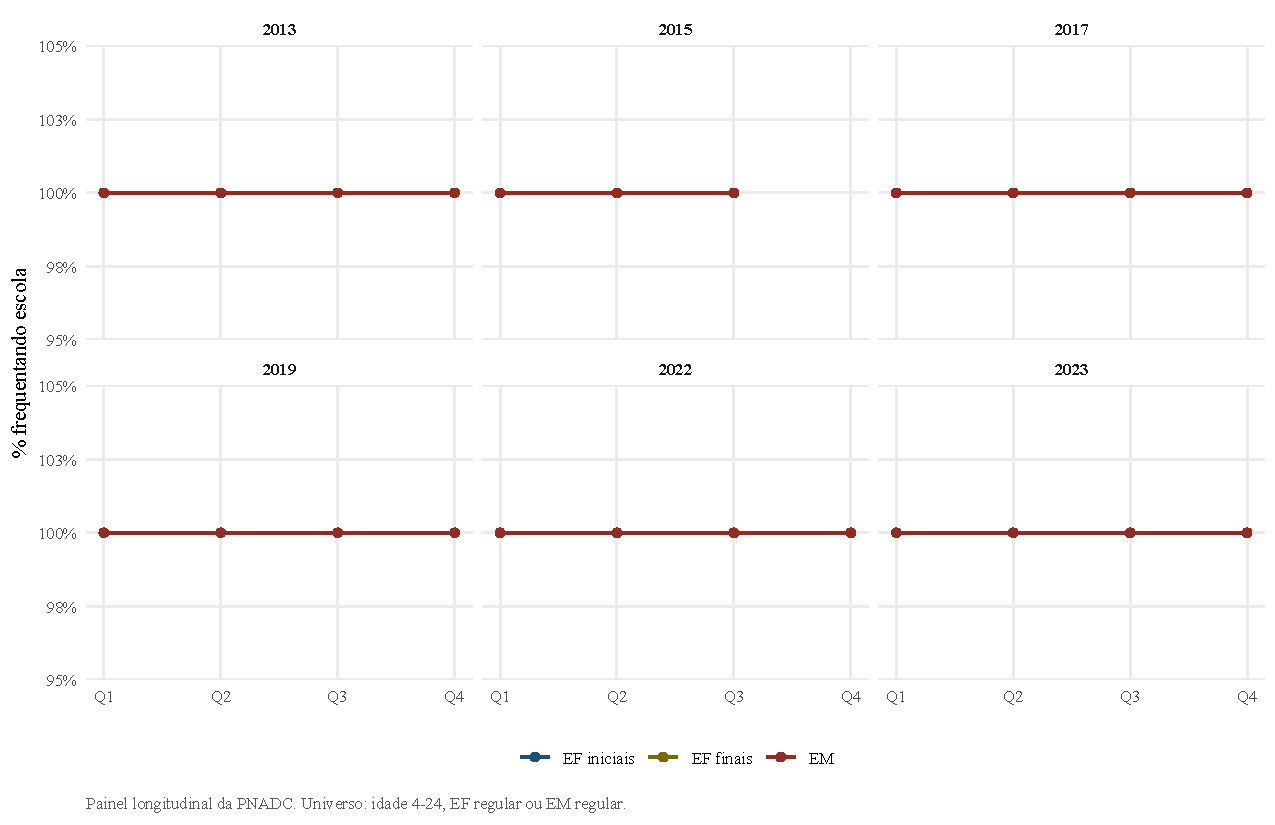
\includegraphics[width=0.95\textwidth]{../DataWork/5_Figures/output/F7_freq_por_trimestre.pdf}
\caption{Percentual de alunos frequentando escola por trimestre, por
macroetapa, anos selecionados.}
\label{fig:freq_trimestre}
\figurenote{Universo: idade quatro a vinte e quatro anos no painel
PNADC, em EF regular ou EM regular. O percentual de frequência é
calculado dentro de cada combinação $($Ano, Trimestre, macroetapa$)$
ponderado pelo peso amostral.}
\end{figure}

A Figura~\ref{fig:cohort_fluxo} replica, com dados da PNADC
trimestral, o exercício de \citet{Fernandes2011_atratividade},
originalmente realizado com dados mensais da PME. Mostramos o índice
de matrículas, normalizado a cem no início de cada série, ao longo
de dezesseis trimestres, para pseudocoortes que entram no oitavo ano
do EF em diferentes anos calendário e progridem até o terceiro ano
do EM. As linhas verticais tracejadas marcam as transições entre
séries, em janeiro do ano seguinte. O Painel A considera todos os
alunos, enquanto o Painel B restringe a alunos sem distorção
idade-série.

\begin{figure}[htbp]
\centering
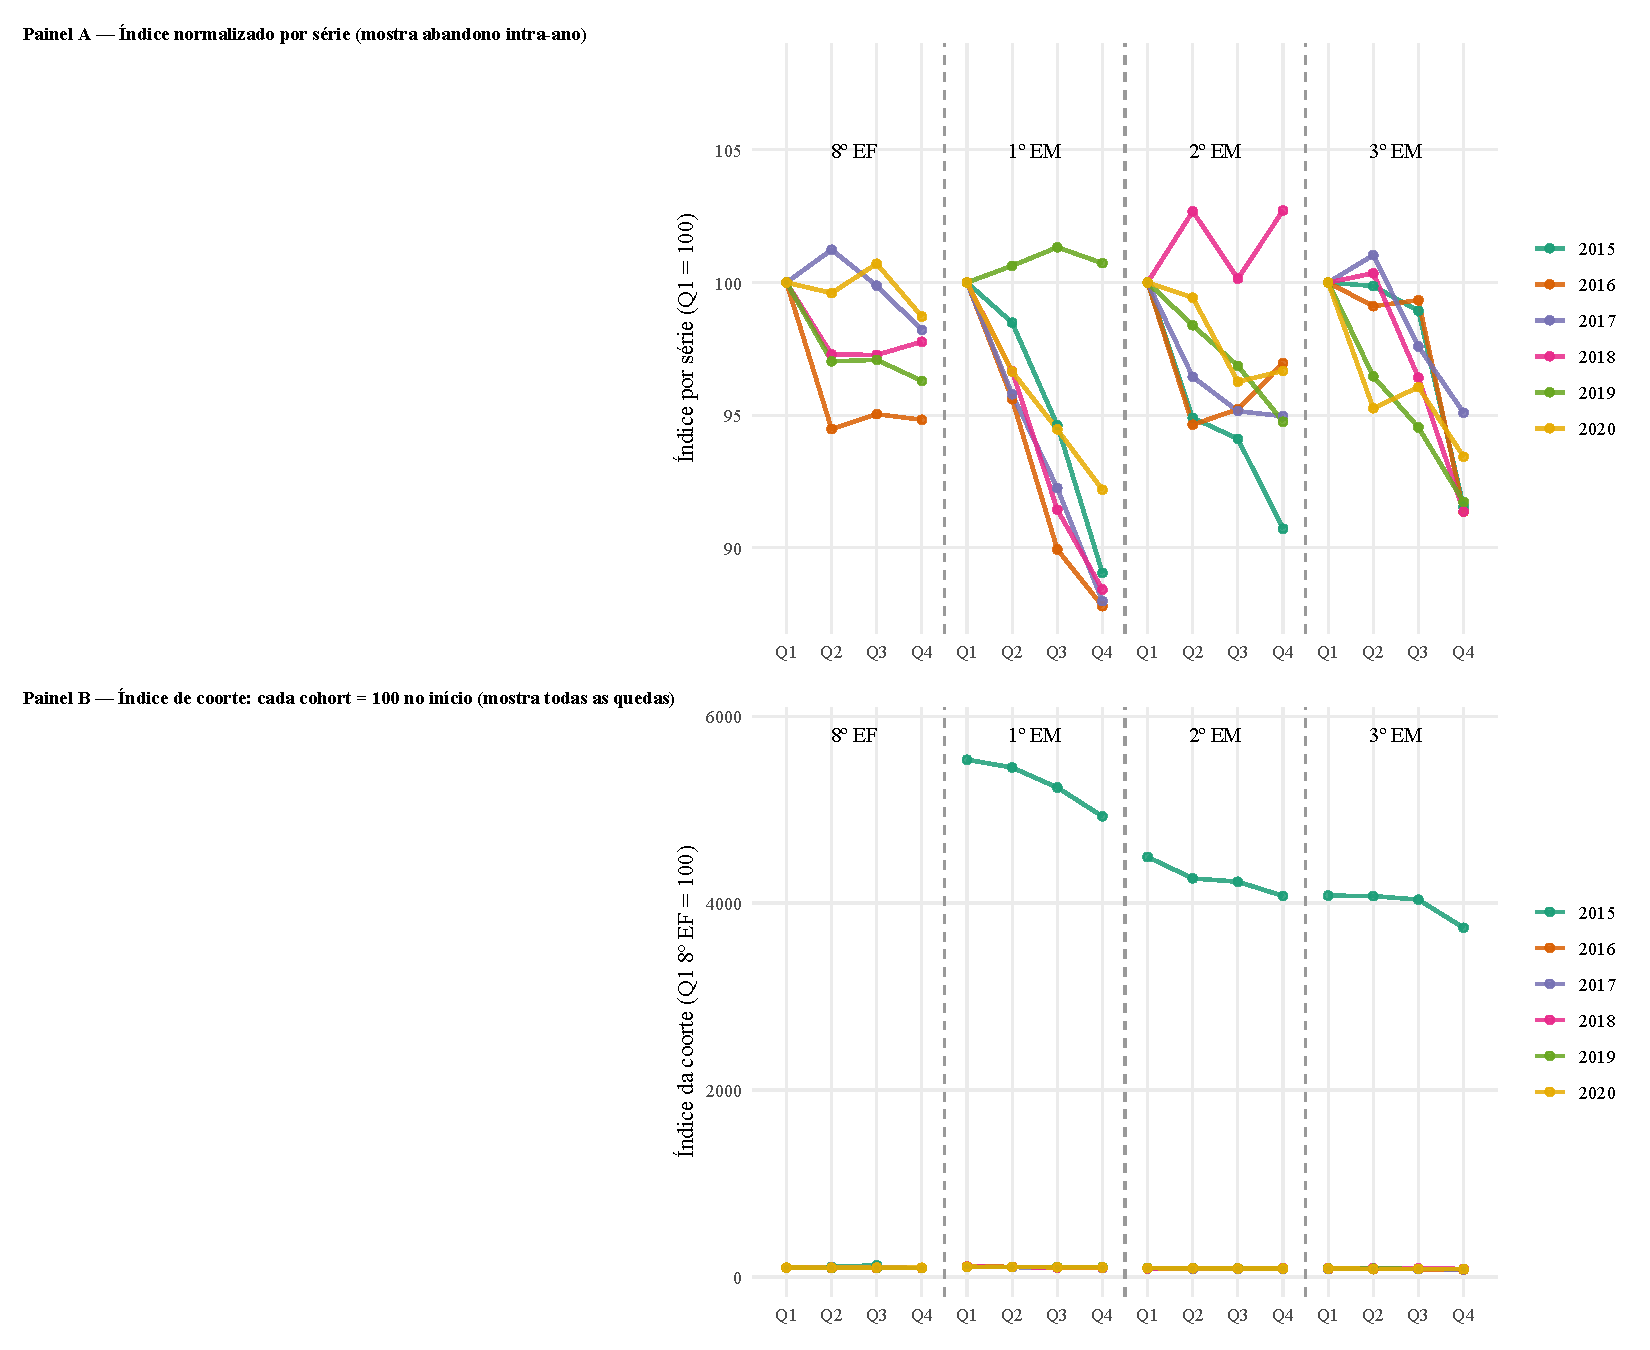
\includegraphics[width=0.95\textwidth]{../DataWork/5_Figures/output/F4_cohort_fluxo.pdf}
\caption{Índice de matrículas por trimestre, ao longo de pseudocoortes
oitavo EF $\to$ terceiro EM (PNADC trimestral, 2013--2024).}
\label{fig:cohort_fluxo}
\figurenote{Cada coorte é definida pela combinação de série-base e
ano calendário de entrada no oitavo EF. O Painel A, com normalização
por série, isto é, cem em $Q_1$ de cada série, evidencia o padrão de
abandono intra-ano. O Painel B, com normalização por coorte, ou seja,
cem em $Q_1$ do oitavo EF, revela todas as quedas, intra-ano
(abandono) e entre séries (evasão, repetência e migração para EJA).
Reproduz e estende o exercício de \citet{Fernandes2011_atratividade}.}
\end{figure}

Três padrões emergem da figura. Em primeiro lugar, no Painel A, a
queda intra-ano dentro de cada série é modesta no oitavo EF e
amplifica-se progressivamente no ensino médio, confirmando o padrão
documentado por \citet{Fernandes2011_atratividade}, em que o
abandono cresce com a idade e com a série. Em segundo lugar, no
Painel B, fica visível que a maior parte da atrição ocorre nas
transições entre séries, isto é, nos saltos verticais nas linhas
tracejadas, e não dentro de cada ano, padrão consistente com o
gargalo histórico do ensino médio brasileiro
\citep{Klein2006_educacao, IMDS_PereiraA002}. Por fim, em terceiro
lugar, ao final dos dezesseis trimestres, o índice da coorte
(Painel B) está em torno de 40\% a 60\% do nível inicial, dependendo
da coorte. Ou seja, apenas cerca de metade dos alunos que estavam no
oitavo EF chegam ao terceiro EM três anos depois, diagnóstico que
motiva a agenda de políticas focalizadas como o Pé-de-Meia
\citep{Brasil2024_PeDeMeia}.

Entre 2012 e 2019, observa-se melhoria consistente em todos os
indicadores do EF. A promoção no EF iniciais sobe de 77,3\% em 2012
para 85,5\% em 2019, e a repetência cai de 17,0\% para 11,8\%. No
EM, a promoção cresce mais modestamente, de 47,6\% em 2012 para
50,4\% em 2019, com a evasão estável em torno de 24\% a 26\%. A
pandemia de COVID-19 interrompe a melhoria. Em 2020, no EF iniciais,
a promoção cai abruptamente para 75,8\% e a repetência sobe para
21,6\%, inversão dramática provavelmente associada às políticas de
aprovação automática ou de suspensão da aprovação adotadas de modo
heterogêneo entre estados e municípios durante a suspensão de aulas
presenciais. Os números de 2020 e 2021 não devem ser interpretados
como piora real do aprendizado, pois refletem rupturas
administrativas no conceito de aprovação. A partir de 2022, observa-se
retomada parcial, mas os níveis de promoção do EF iniciais em 2023
(72,4\%) ainda não retornaram ao patamar pré-pandemia.

O ano de 2024 marca a entrada do Pé-de-Meia
\citep{Brasil2024_PeDeMeia} no calendário escolar, com pagamento a
partir de março. A medida visa, entre outros objetivos, reduzir a
evasão no EM público. Como o programa só começa em 2024, ainda é
cedo para identificar seus efeitos com a janela do painel da PNADC,
pois a transição 2024--2025 ainda não está disponível. A
monitorização desse impacto será imediatamente possível assim que o
IBGE disponibilizar a PNADC 2025Q1. Os anos de 2020 e 2021 são
tratados separadamente nas tabelas e figuras por duas razões. Em
primeiro lugar, o IBGE conduziu parte das entrevistas por telefone
durante o pico da pandemia, o que pode introduzir viés de
não-resposta diferencial. Em segundo lugar, o fechamento de escolas
reduziu a comparabilidade do conceito de frequentar escola, uma vez
que alunos podiam estar matriculados mas sem aulas presenciais. Nas
figuras, o intervalo 2020--2021 aparece sombreado, e nas tabelas
esses anos vêm marcados com $\dagger$. As séries de média multianual
reportadas na Seção~\ref{sec:heterogeneidade} excluem 2020 e 2021 do
cálculo da média 2018--2023, restringindo-se aos anos pré-COVID
(2018 e 2019) e pós-COVID (2022 e 2023).
